\documentclass[aspectratio=169]{beamer}
\usepackage[utf8]{inputenc}
\usepackage{multimedia}  % for videos
\usepackage{hyperref}
\usepackage[sfdefault]{noto}  % define font: noto sans
\usepackage{enumitem}
\setlist[itemize]{noitemsep, topsep=0pt, label=\usebeamerfont*{itemize item}
    \usebeamercolor[fg]{itemize item}
    \usebeamertemplate{itemize item}}

%\usetheme{Madrid}
%\usecolortheme{lily}
\usetheme[progressbar=frametitle]{metropolis}
\setbeamertemplate{frame numbering}[fraction]  % to add total number of pages
\metroset{background=dark}

\definecolor{defcolor}{RGB}{245, 10, 10}  % define custom color

% change colors of the theme
\setbeamercolor{palette primary}{bg=white, fg=black}
\setbeamercolor{background canvas}{parent=palette primary}
\setbeamercolor{normal text}{fg=black}
\setbeamercolor{progress bar}{use=palette primary, fg=defcolor}


% refs
\usepackage[backend=bibtex, style=numeric]{biblatex}
\addbibresource{refs.bib}
\AtBeginBibliography{\small}  % change font size for the refs

% footnote and page number on the same line & logo
\setbeamertemplate{footline}{}
\setbeamertemplate{logo}{
 \usebeamercolor[fg]{footline}
 \usebeamerfont{page number in head/foot}
 \usebeamertemplate*{frame numbering}
 }


\title{ Using Graph Neural Networks as a Preconditioner (GNP) in Soil–Structure Interaction}
\subtitle{}
\author{
    Aron Noordam
    }


\date{\today}

\begin{document}

% ####################################################################
\begin{frame}[plain]{}
\titlepage
\end{frame}

% ####################################################################
\begin{frame}{Motivation}
	\textbf{Problem:} Soil--structure interaction (SSI)
	
	\medskip
	
	\begin{itemize}
		\item Large stiffness variations in finite element model
		\item $\Rightarrow$ Ill-conditioned systems
		\item $\Rightarrow$ Slow / expensive solvers
	\end{itemize}
	
	\medskip
	
	\alert{Goal: Improve solver efficiency}
\end{frame}


% ####################################################################

\begin{frame}{Preconditioning Concept}
	
	Typically in FEM, we solve:
	\[
	Ax = b
	\]
	
	\medskip
	
	With preconditioner, we solve:
	\[
	M^{-1}Ax = M^{-1}b
	\]
	
	\medskip
	
	\begin{block}{Goal}
		Construct $M$ such that $M \approx A^{-1}$
	\end{block}
	
	\medskip
	
	\begin{itemize}
		\item Improves conditioning of the system
		\item Reduces number of solver iterations
	\end{itemize}
\end{frame}

%------------------------------------------------

\begin{frame}{Approach}
	We compare three approaches:
	
	\begin{itemize}
		\item No preconditioning
		\item Jacobi preconditioner
		\item \textbf{Graph Neural Network Preconditioner (GNP)}
	\end{itemize}
	
	\medskip
	
	Test cases:
	
	\begin{itemize}
		\item Well-conditioned system
		\item Ill-conditioned system
	\end{itemize}
	
	\medskip
	
\end{frame}


%------------------------------------------------

\begin{frame}{Approach}
	 \framesubtitle{Linear Solver}
	
	\textbf{Conjugate Gradient (CG)}
	
	\medskip
	
	\begin{itemize}
		\item Iterative solver for symmetric positive definite matrices
		\item Widely used in FEM applications
	\end{itemize}
	
	\medskip
	
	Stopping criteria:

	\medskip
	
	\begin{itemize}
		\item $\|r\| < 10^{-12}$
		\item Maximum iterations: 1000
	\end{itemize}
	

\end{frame}

%------------------------------------------------

\begin{frame}{Approach}
	\framesubtitle{Preconditioner}
	\textbf{Jacobi Preconditioner}
	
	
	\[
	M = D
	\]
	
	\medskip
	
	\begin{itemize}
		\item Uses only diagonal entries of $A$
		\item Very cheap to compute and apply
	\end{itemize}
	
	\medskip
	
	\begin{block}{Limitation}
		Does not capture coupling between degrees of freedom
	\end{block}
	
\end{frame}

%------------------------------------------------

\begin{frame}{Approach}
		\framesubtitle{Preconditioner}
	\textbf{GNN Preconditioner (GNP) \cite{Chen_2024}}
	
	\medskip
	
	\textbf{Key idea: Learn the inverse operator}
	
	\medskip
	
	\begin{block}{Training data}
		Pairs of vectors: $(b, x)$ 
	\end{block}
	
	\medskip
	
	Model learns:
	
	\[
	Mb \rightarrow x
	\]
	
	\medskip
	
	\begin{itemize}
		\item Based on Graph Convolutional Networks (GCN)
		\item Captures global interactions beyond diagonal approximation
	\end{itemize}
	

\end{frame}


%------------------------------------------------

\begin{frame}{Approach}
	\framesubtitle{Computational Setup}

	\begin{itemize}
		\item GNP training performed on GPU
		\item Linear solves also GPU-accelerated
	\end{itemize}
	
	\medskip
	
	\begin{block}{Hardware}
		NVIDIA RTX A1000 6GB Laptop GPU
	\end{block}
	

\end{frame}

%------------------------------------------------

\begin{frame}{Results Overview}
	Two test cases:
	
	\begin{itemize}
		\item \textbf{Case 1:} Small, well-conditioned system
		\item \textbf{Case 2:} Large, ill-conditioned system
	\end{itemize}
	
	\medskip
	
	We evaluate:
	
	\begin{itemize}
		\item Convergence (CG iterations)
		\item Computational time
	\end{itemize}
	

\end{frame}

%------------------------------------------------

\begin{frame}{Case 1: Problem Setup}
	\textbf{Small scale, well-conditioned system}
	
	 \begin{columns}
		\begin{column}{0.45\textwidth}
			\begin{itemize}
			\item Size: $3509 \times 3509$
			\item Non-zeros: $2.26 \times 10^5$
			\item Condition number: $\sim 9.0 \times 10^2$
			\end{itemize}
		\end{column}
		\begin{column}{0.55\textwidth}
			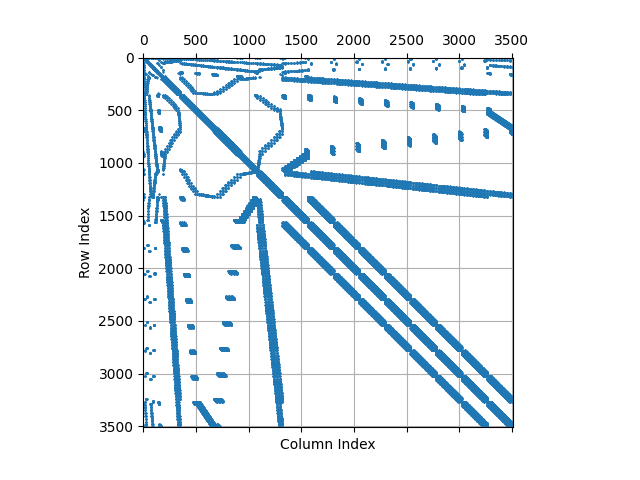
\includegraphics[width=1.0\linewidth]{static/3_5k_x_3_5k_matrix_sparsity.png}

		\end{column}
	\end{columns}
	
	
\end{frame}

%------------------------------------------------

\begin{frame}{Case 1: GNP Training}
	
	\begin{columns}
		\begin{column}{0.45\textwidth}
			\begin{itemize}
				\item Epochs: 2000
				\item Training time: 71 seconds
				\item Minimum loss: $8.5 \times 10^{-3}$
			\end{itemize}
		\end{column}
		\begin{column}{0.55\textwidth}
			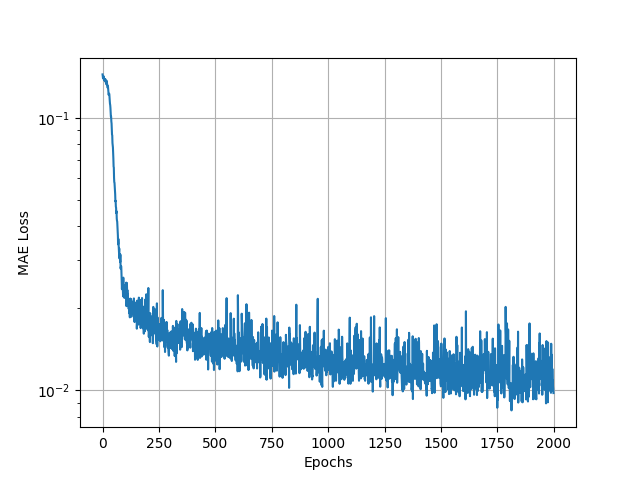
\includegraphics[width=1.0\linewidth]{static/3_5k_x_3_5k_matrix_training.png}
			
		\end{column}
	\end{columns}
	
\end{frame}

%------------------------------------------------

\begin{frame}{Case 1: Performance}
	\textbf{Observations:}
	
	\medskip
	
	\begin{itemize}
		\item GNP lowers iterations significantly
		\item BUT increases total computation time
	\end{itemize}
	
	\medskip
	
	\begin{columns}
		\column{0.5\linewidth}
		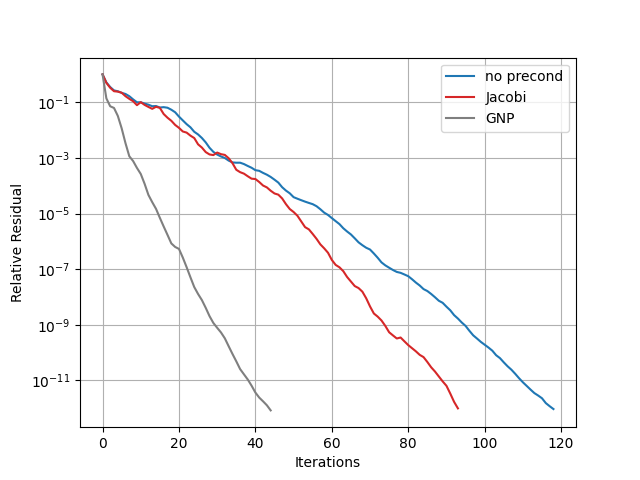
\includegraphics[width=\linewidth]{static/3_5k_x_3_5k_matrix_solver.png}
		
		\column{0.5\linewidth}
		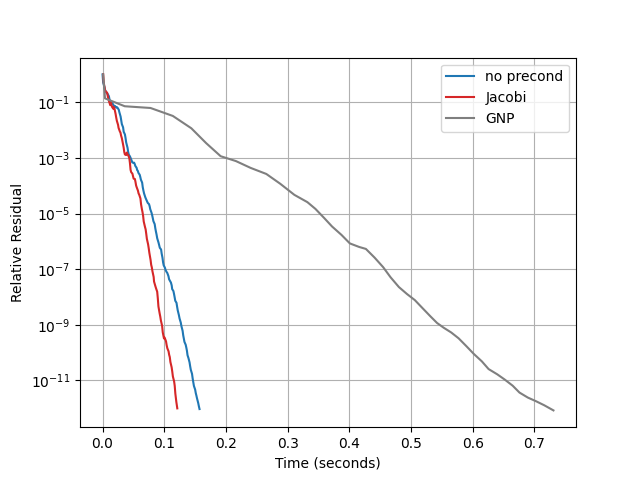
\includegraphics[width=\linewidth]{static/3_5k_x_3_5k_matrix_time.png}
	\end{columns}
	
\end{frame}

%------------------------------------------------

\begin{frame}{Case 2: Problem Setup}
	\textbf{Large-scale, ill-conditioned system}
	
	 \begin{columns}
		\begin{column}{0.45\textwidth}
			\begin{itemize}
				\item Size: $60{,}468 \times 60{,}468$
				\item Non-zeros: $2.43 \times 10^6$
				\item Condition number: $\sim 2.6 \times 10^9$
			\end{itemize}
		\end{column}
		\begin{column}{0.55\textwidth}
			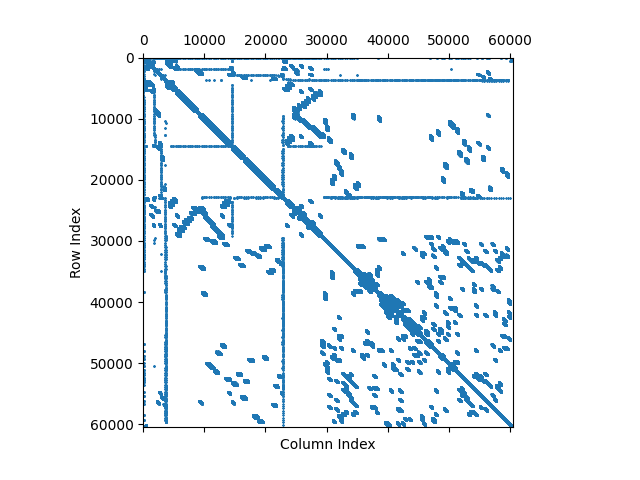
\includegraphics[width=1.0\linewidth]{static/60k_x_60k_matrix_sparsity.png}
			
		\end{column}
	\end{columns}
	
\end{frame}

%------------------------------------------------

\begin{frame}{Case 2: GNP Training}
	\begin{columns}
		\begin{column}{0.45\textwidth}
			\begin{itemize}
				\item Epochs: 4000
				\item Training time: 24 minutes
				\item Minimum loss: $4.2 \times 10^{-4}$
			\end{itemize}
	
		\end{column}
		\begin{column}{0.55\textwidth}
	
			\begin{center}
				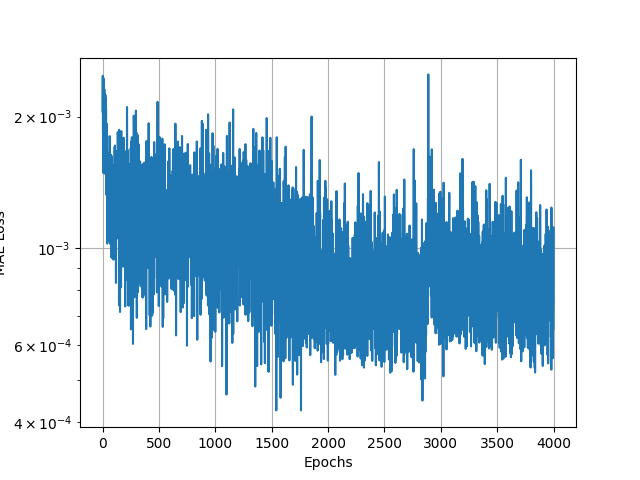
\includegraphics[width=1\linewidth]{static/60k_x_60k_matrix_training.png}
			\end{center}
		\end{column}
	\end{columns}
\end{frame}

%------------------------------------------------

\begin{frame}{Case 2: Performance}
	\textbf{Observations:}
	
	\medskip
	
	\begin{itemize}
		\item GNP fails to converge within 1000 iterations
		\item Worse than \textbf{no preconditioner}
		\item Jacobi significantly improves convergence
	\end{itemize}
	
	\medskip
	
	\begin{columns}
		\column{0.5\linewidth}
		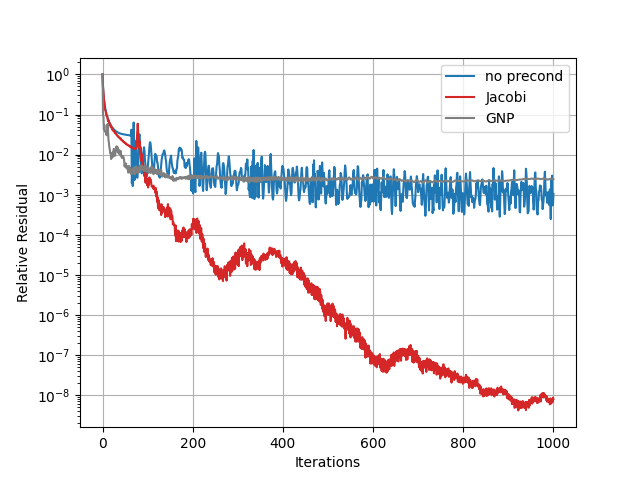
\includegraphics[width=\linewidth]{static/60k_x_60k_matrix_solver.png}
		
		\column{0.5\linewidth}
		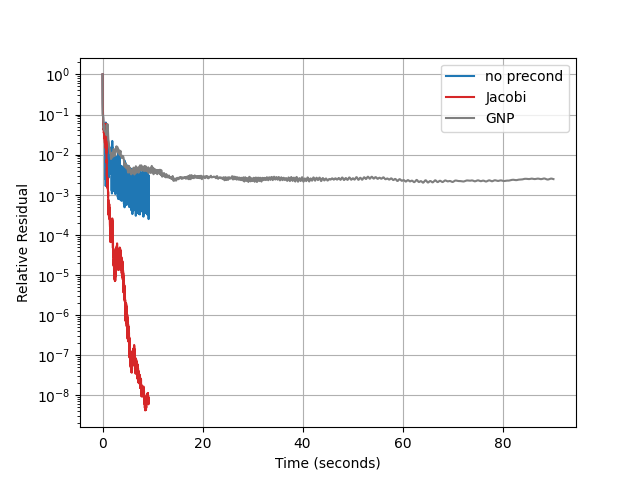
\includegraphics[width=\linewidth]{static/60k_x_60k_matrix_time.png}
	\end{columns}
	
	\medskip
	
	\alert{GNP does not scale to difficult systems}
\end{frame}

%------------------------------------------------

\begin{frame}{Key Findings}
	\begin{itemize}
		\item Training cost $\ggg$ solve cost (both cases)
		\item GNP reduces iterations only for easy problems
		\item No benefit in total runtime
	\end{itemize}
	
	\medskip
	
	\begin{block}{Critical limitation}
		GNP must be retrained for each new system
	\end{block}
\end{frame}

%------------------------------------------------

\begin{frame}{Conclusion}
	\begin{itemize}
		\item For small / well-conditioned systems:
		\begin{itemize}
			\item Fewer iterations with GNP
			\item But slower overall than Jacobi
		\end{itemize}
		
		\medskip
		
		\item For large / ill-conditioned systems:
		\begin{itemize}
			\item GNP fails to improve convergence
		\end{itemize}
	\end{itemize}
	
	\medskip
	
	\begin{block}{Final Verdict}
		No clear practical benefit of GNP for soil-structure interaction problems
	\end{block}
	

\end{frame}

%------------------------------------------------

\begin{frame}[allowframebreaks, noframenumbering]
	\printbibliography
\end{frame}

\end{document}

